% Autor: Leonhard Segger, Alexander Neuwirth
% Datum: 2017-10-30
\documentclass[
	% Papierformat
	a4paper,
	% Schriftgröße (beliebige Größen mit „fontsize=Xpt“)
	12pt,
	% Schreibt die Papiergröße korrekt ins Ausgabedokument
	pagesize,
	% Sprache für z.B. Babel
	ngerman
]{scrartcl}

% Achtung: Die Reihenfolge der Pakete kann (leider) wichtig sein!
% Insbesondere sollten (so wie hier) babel, fontenc und inputenc (in dieser
% Reihenfolge) als Erstes und hyperref und cleveref (Reihenfolge auch hier
% beachten) als Letztes geladen werden!

% Silbentrennung etc.; Sprache wird durch Option bei \documentclass festgelegt
\usepackage{babel}
% Verwendung der Zeichentabelle T1 (Sonderzeichen etc.)
\usepackage[T1]{fontenc}
% Legt die Zeichenkodierung der Eingabedatei fest, z.B. UTF-8
\usepackage[utf8]{inputenc}
% Schriftart
\usepackage{lmodern}
% Zusätzliche Sonderzeichen
\usepackage{textcomp}

% Mathepaket (intlimits: Grenzen über/unter Integralzeichen)
\usepackage[intlimits]{amsmath}
% Ermöglicht die Nutzung von \SI{Zahl}{Einheit} u.a.
\usepackage{siunitx}
% Zum flexiblen Einbinden von Grafiken (\includegraphics)
\usepackage{graphicx}
% Abbildungen im Fließtext
\usepackage{wrapfig}
% Abbildungen nebeneinander (subfigure, subtable)
\usepackage{subcaption}
% Funktionen für Anführungszeichen
\usepackage{csquotes}
% Zitieren, Bibliographie
\usepackage{biblatex}


% Zur Darstellung von Webadressen
\usepackage{url}
%chemische Formeln
\usepackage[version=4]{mhchem}
% siunitx: Deutsche Ausgabe, Messfehler getrennt mit ± ausgeben
\usepackage{floatrow}
\floatsetup[table]{capposition=top}
\usepackage{float}
% Verlinkt Textstellen im PDF-Dokument
\usepackage[unicode]{hyperref}
% "Schlaue" Referenzen (nach hyperref laden!)
\usepackage{cleveref}
\sisetup{
	locale=DE,
	separate-uncertainty
}
\bibliography{6Mi_E4_24-01-2018_References}

\begin{document}
	
	\begin{titlepage}
		\centering
		{\scshape\LARGE Versuchsbericht zu \par}
		\vspace{1cm}
		{\scshape\huge E4 - Kennlinien \par} %TODO Anpasen
		\vspace{2.5cm}
		{\LARGE Gruppe 6Mi \par}
		\vspace{0.5cm}
		
		{\large Alexander Neuwirth (E-Mail: a\_neuw01@wwu.de) \par}
		{\large Leonhard Segger (E-Mail: l\_segg03@uni-muenster.de) \par}
		\vfill
		
		durchgeführt am 24.01.2018\par %TODO Anpassen
		betreut von\par
		{\large Christoph Angrick} %TODO Anpassen
		
		\vfill
		
		{\large \today\par}
	\end{titlepage}
	\tableofcontents
	\newpage

	%TODO mehr TODO in Default	

	\section{Kurzfassung}
	In diesem Versuch wurden die Kennlinien verschiedener elektrischer Bauteile erfasst.
	Dazu wurde die Stromstärke in Abhängigkeit von der Spannung für eine Diode in Durchlassrichtung, eine Zenerdiode in Sperr- und Durchlassrichtung, eine Glühlampe, eine Glimmlampe und ein NTC-Widerstand gemessen. 
	Des Weiteren wurde der Widerstand eines Metalldrahts durch eine Wheatstonesche Brücke unter Variation seiner Temperatur untersucht.

	Unsere Hypothesen, dass mit der Spannung auch die Stromstärke für jedes Bauteil monoton steigt und dass die Löschspannung der Glimmlampe kleiner als die Zündspannung ist, konnten im Experiment bestätigt werden.
	Die gemessene Löschspannung war \SI{84\pm 0,14}{V} und die Zündspannung \SI{105\pm3,8}{V}.

	Von dem NTC-Widerstand haben wir erwartet, dass der Widerstand mit der Temperatur abnimmt und sich mit steigender Stromstärke erhitzt. 
	Auch die hieraus resultierende Abnahme des Widerstands mit der Spannung wurde im Experiment beobachtet. %old: nachgewiesen
	Unsere Hypothese für den Widerstand des Metalldrahts bei unterschiedlichen Temperaturen lautet, dass der Widerstand unabhängig von der vorherigen Temperatur sein sollte. 
	Das heißt, es sollte sich beim Erhitzten und beim Abkühlen der selbe Temperaturkoeffizient $\alpha$ ergeben.
	Die von uns gemessenen Temperaturkoeffizienten betragen bei steigender Temperatur \SI{0,00905\pm 0,00011}{} und bei fallender Temperatur \SI{0,0092\pm 0,000095}{}.

	%TODO Hypothese	und deren Ergebnis
	%TODO Ergebnisse, auch Zahlen, mindestens wenn's halbwegs Sinn ergibt
	%TODO Was wurde gemacht
	
	\section{Methoden}
	%TODO Bilder von der Website klauen
	Um die Kennlinien verscheidener Bauteile zu untersuchen, wurde jeweils ein Stromkreis nach \cref{Aufbau} aufgebaut.
	Für die Diode (a), Zenerdiode (b), und den NTC-Widerstand (d) wurden die Stromstärke $I$ in Abhängigkeit von der Spannung $U$ aus dem Interval \SI{0}{V} bis \SI{20}{V} untersucht. 
	Für die Glühlampe wurde eine kleinerer Bereich von Spannungen angelegt (\SI{0}{V} bis \SI{3}{V}) und für die Glimmlampe eine größerer (\SI{0}{V} bis \SI{150}{V}).
	Mit zwei Multimetern wurde die Spannung und die Stromstärke ermittelt.
	Die maximale Stromstärke der Spannungsquelle war ca. \SI{55}{mA}.
	Die Diode wurde nur in Durchlassrichtung und die Zenerdiode in Sperr- und Durchlassrichtung untersucht.
	Beim NTC-Widerstand wurde einige Minuten gewartet bis sich ein konstanter Wert für die Stromstärke eingestellt hat, da sich zunächst ein Temperaturgleichgewicht einstellen musste und sich die Stromstärke währenddessen änderte.

	Im zweiten Teil des Experiments wurde ein Metalldraht in einem Ölbad durch eine Herdplatte erhitzt und danach mit Eis abgekühlt.
	Der Widerstand des Drahtes wurde dabei durch eine Wheatstonesche Brückenschaltung ermittelt (\cref{Wheatstone}).
	Der \SI{11,3}{\Omega}-Widerstand wird so aufgeteilt, dass keine Stromstärke am Amperemeter angezeigt wird.
	Dabei kann der Schalter am \SI{20}{k\Omega}-Widerstand umgelegt werden, um die gemessene Stromstärke möglichst exakt auf Null justieren zu können.
	Mit einem Thermometer wurde die Temperatur des Öls gemessen und in \SI{5}{\celsius} Schritten wurde die Einstellung des verstellbaren Widerstands angepasst und aufgenommen. 
	Ab einer Temperatur von \SI{95}{\celsius} wurde mit Eis abgekühlt und erneut in gleichen Abständen der Widerstand an der Wheatstone Brücke eingestellt und dokumentiert.
	\begin{figure}[H]
		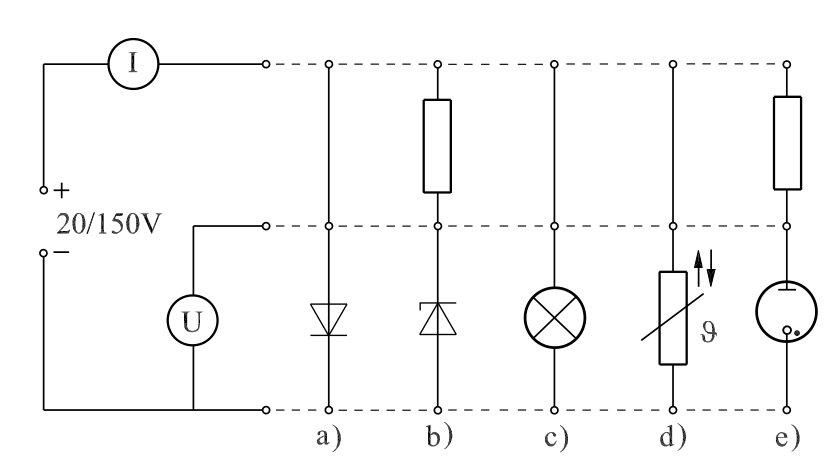
\includegraphics[width=0.7\textwidth]{Aufbau}
		\centering
		\caption{Experimenteller Aufbau zur Bestimmung der Kennlinien.\cite{WWU}} 
		\label{Aufbau}
		\centering
	\end{figure} 	
	\begin{figure}[H]
		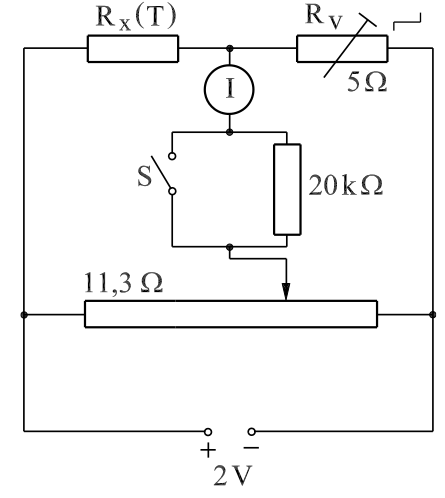
\includegraphics[width=0.5\textwidth]{Wheatstone}
		\centering
		\caption{Wheatstonesche Brückenschaltung. Durch Variation des Mittleren Widerstands kann $R_x$ bestimmt werden.\cite{WWU}} 
		\label{Wheatstone}
		\centering
	\end{figure} 	
	
	\section{Ergebnisse und Diskussion}
	%TODO Datenanalyse -> Überschrift?
	%TODO Unsicherheiten

	\subsection{Beobachtung}
	\subsection{Strom-Spannungs-Charakteristiken}
	Im Folgenden ergibt sich der Fehler der Strom- und Spannungsmessung aus der Unsicherheit durch die Digitalanzeige der verwendeten Multimeter (also rechteckige WDF).
	Da in unterschiedlichen Skalen gemessen wurde, wurde hierfür jeweils die Unsicherheit des Messwerts mit der größten Skala verwendet.
	Die Abhängigkeit der Stromstärke von der Spannung der verwendeten Diode in Durchlassrichtung wurde in \cref{Diode} dargestellt.
	\begin{figure}[H]
		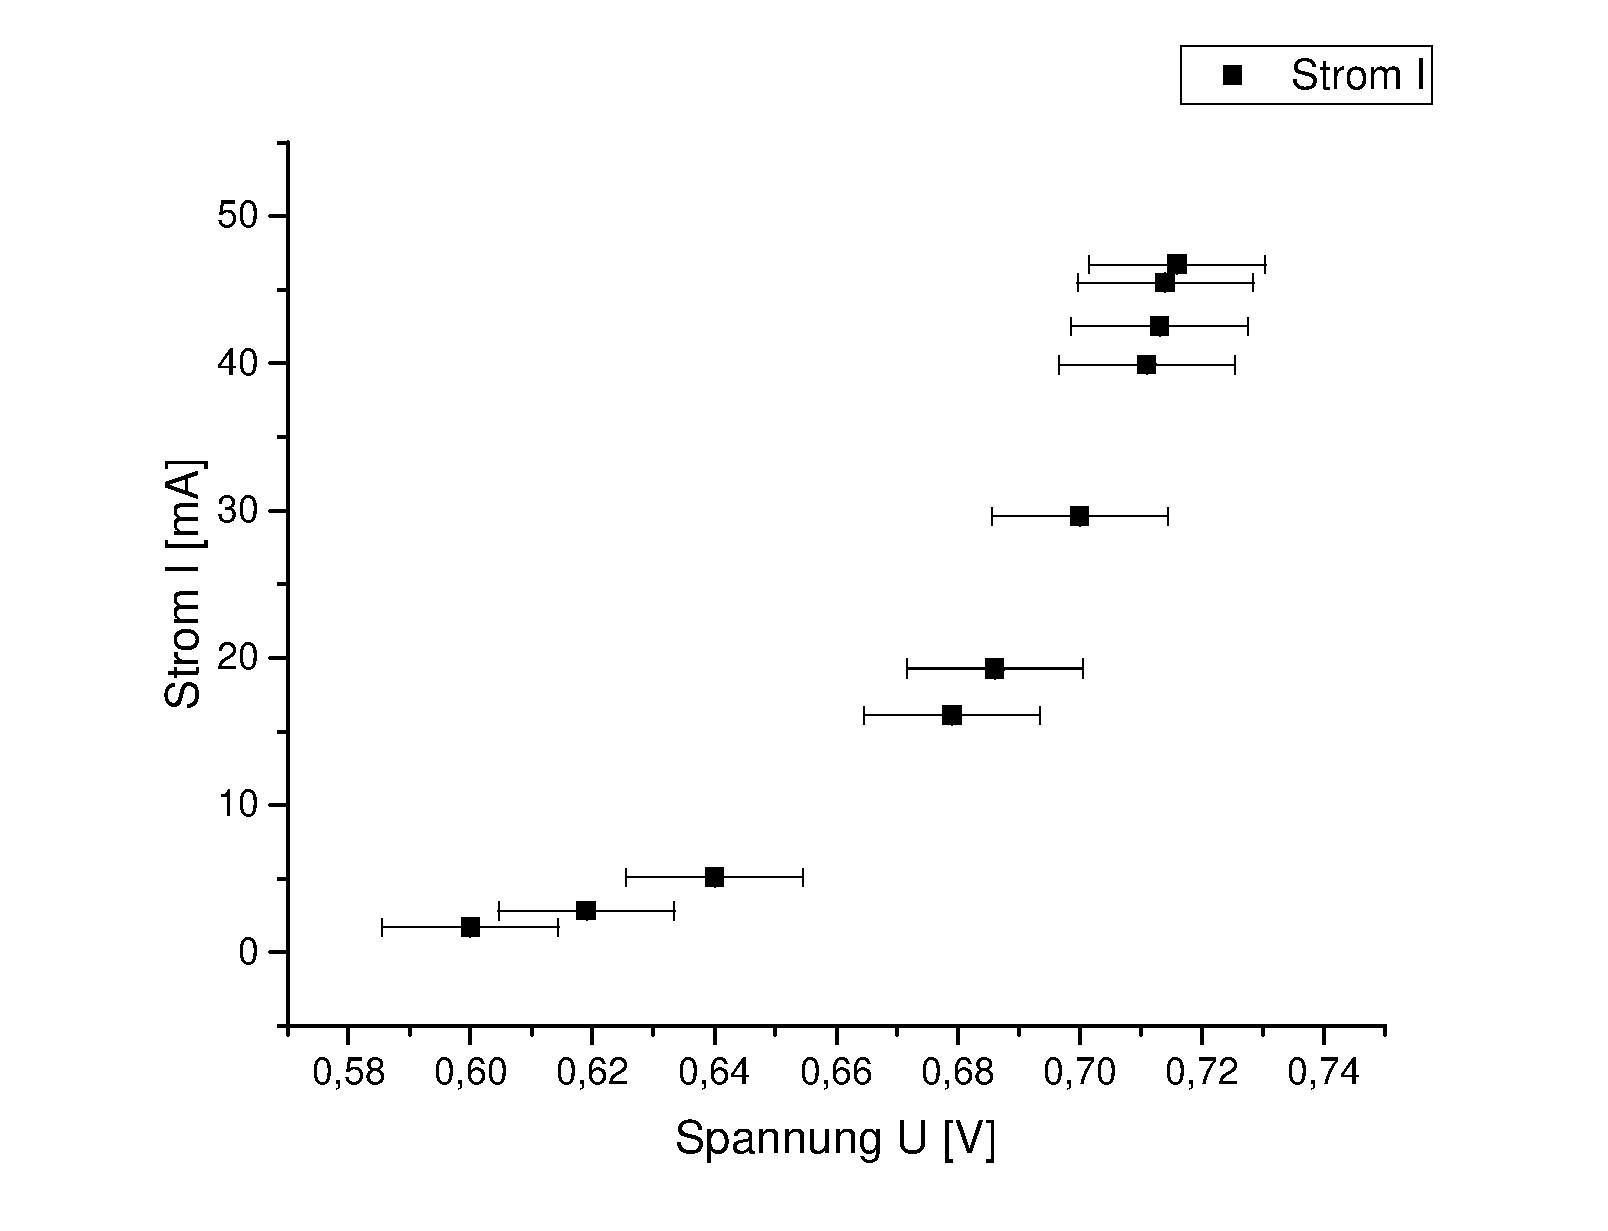
\includegraphics[width=0.7\textwidth]{Diode}
		\centering
		\caption{Hier ist die Stromstärke  gegen die Spannung bei Betrieb einer Diode aufgetragen. Die Unsicherheit in y-Richtung ist kleiner als die Symbolgröße.}
		\label{Diode}
		\centering
	\end{figure} 
	In \crefrange{Zener_Durch}{Zener_Sperr} wurden die experimentell ermittelten Kennlinien der Zenerdiode in Durchfluss- und Sperrrichtung aufgetragen.
	\begin{figure}[H]
		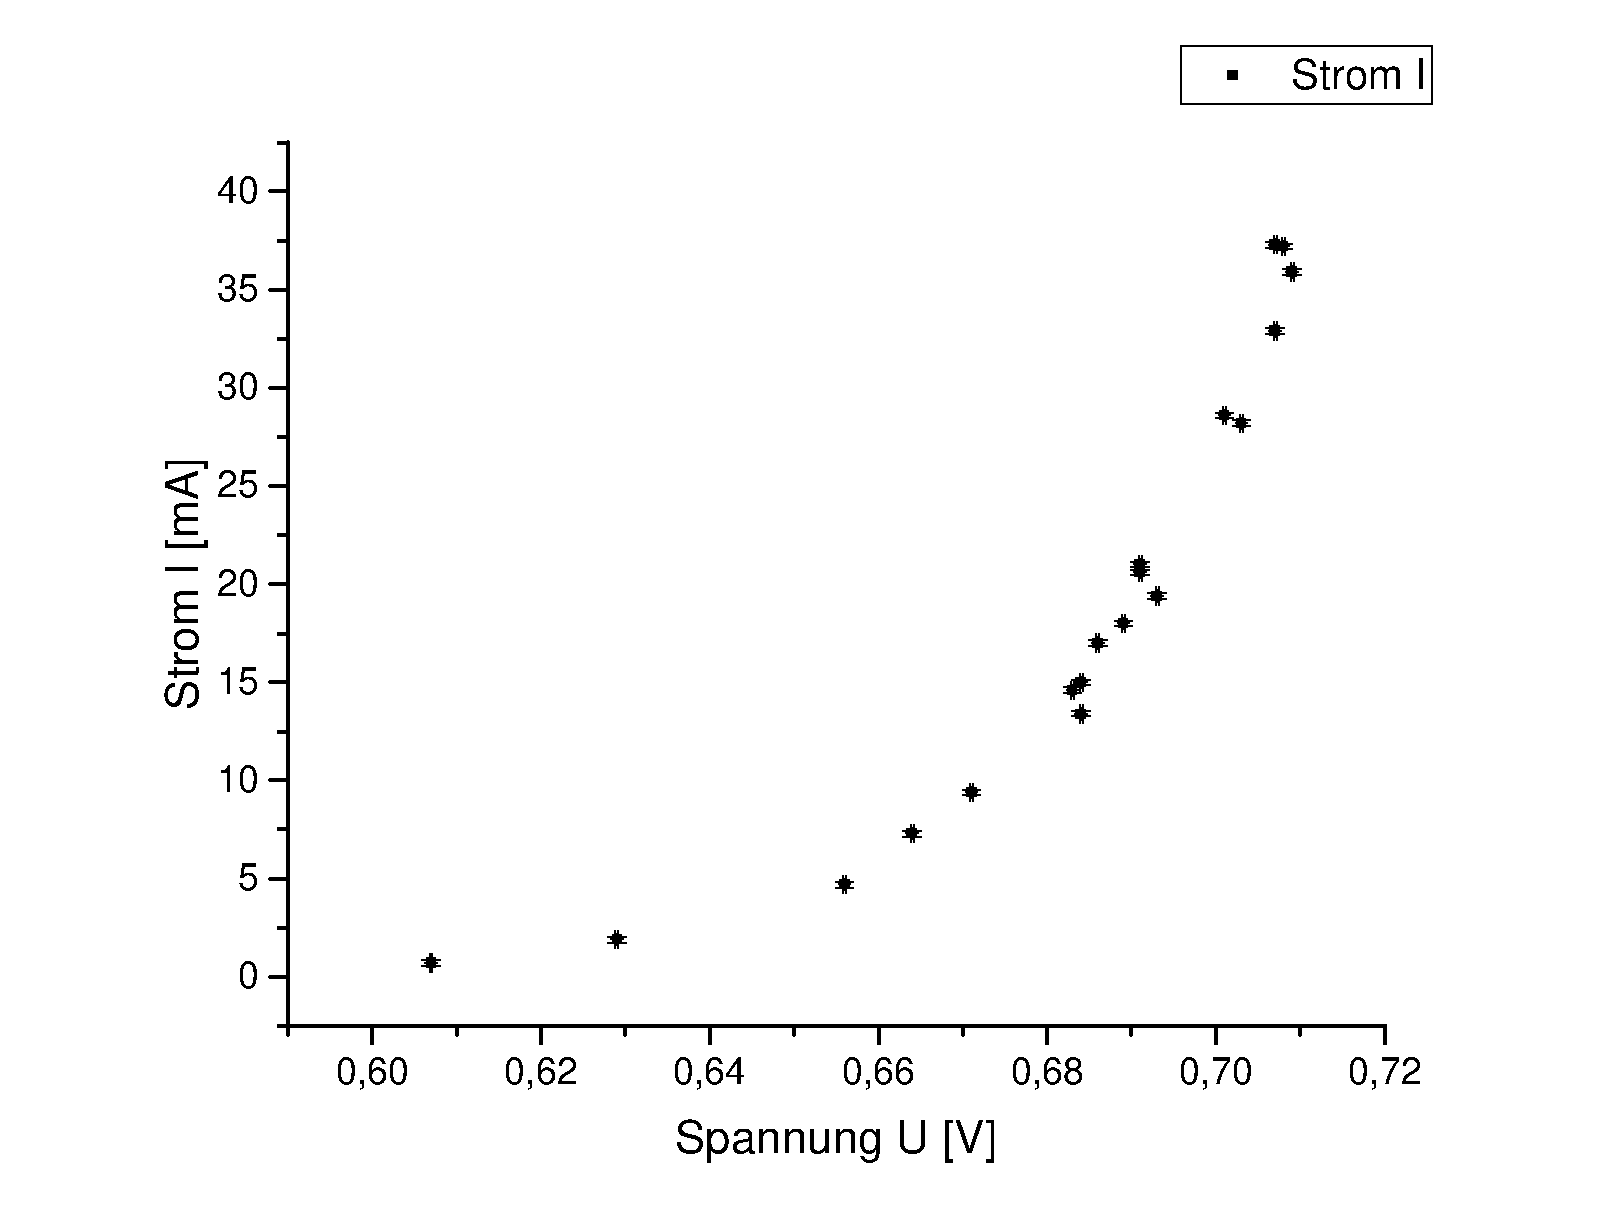
\includegraphics[width=0.7\textwidth]{Zener_Durch}
		\centering
		\caption{Hier ist die Stromstärke  gegen die Spannung bei Betrieb einer Zenerdiode in Durchflussrichtung aufgetragen. Die Unsicherheit ist kleiner als die Symbolgröße.}
		\label{Zener_Durch}
		\centering
	\end{figure}
	\begin{figure}[H]
		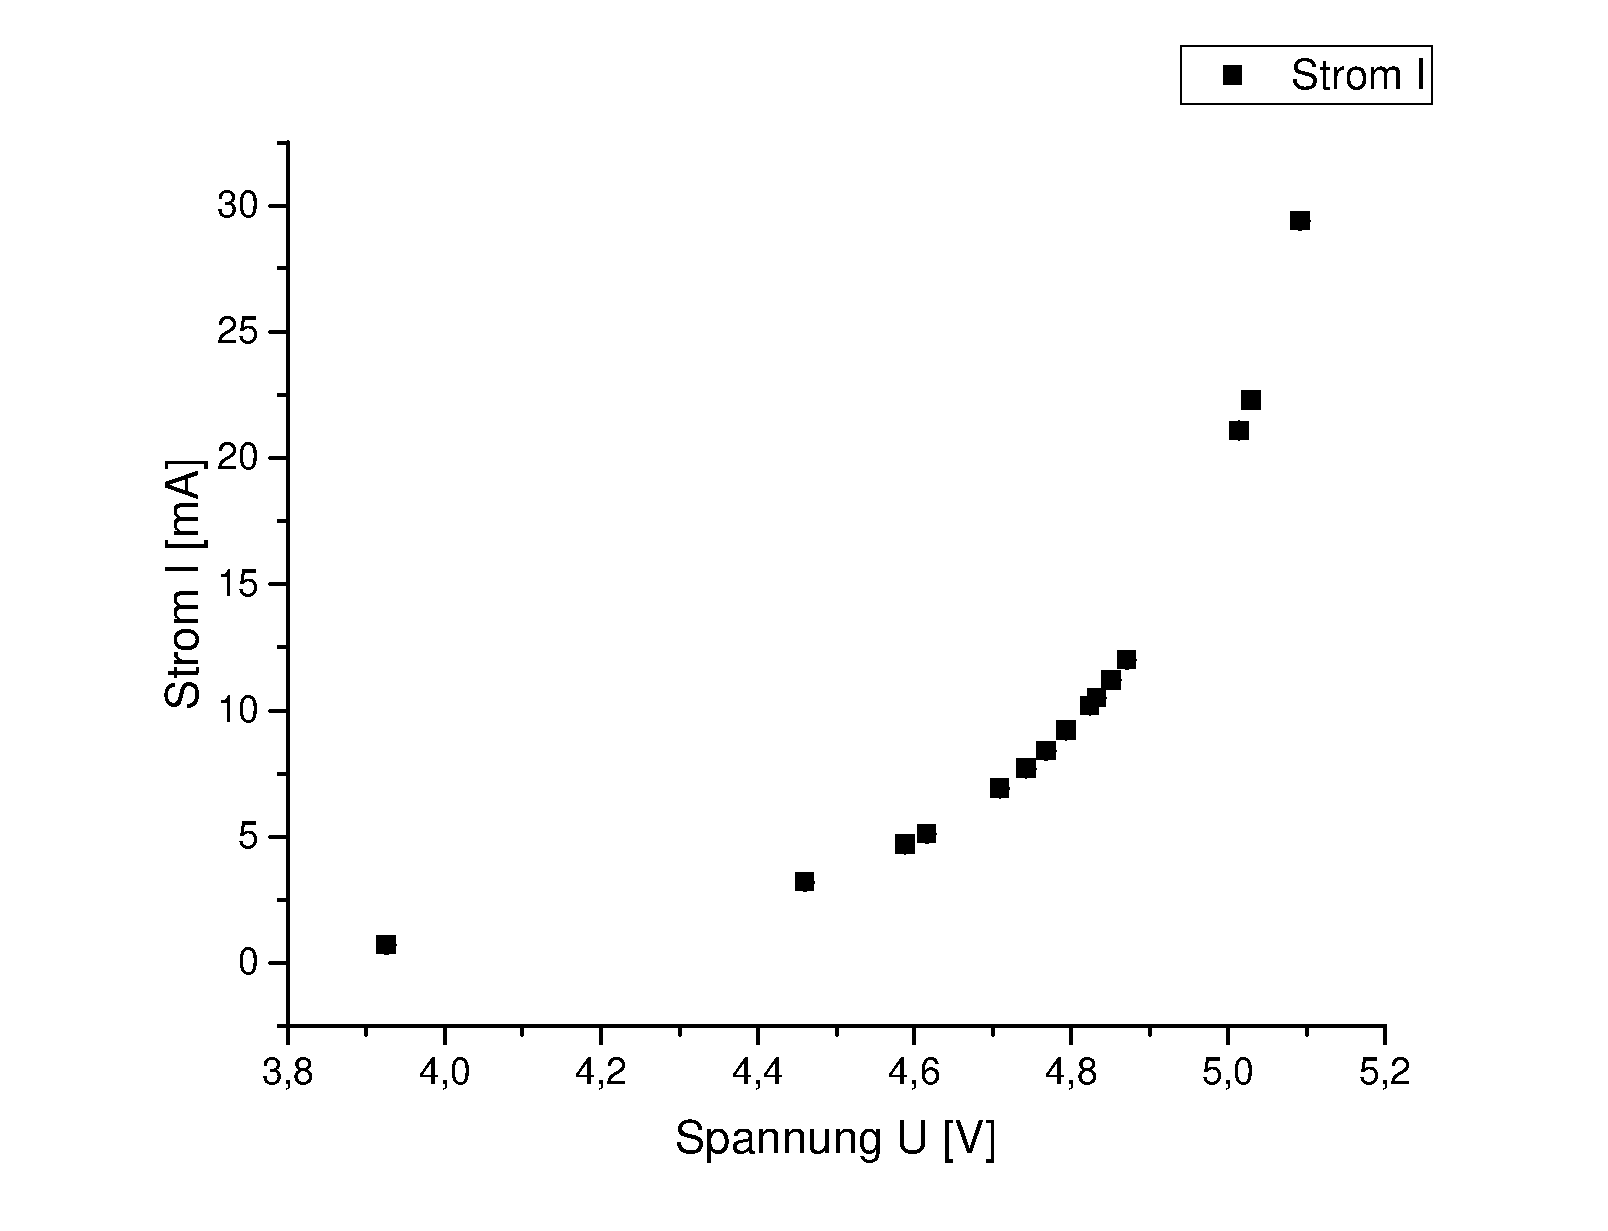
\includegraphics[width=0.7\textwidth]{Zener_Sperr}
		\centering
		\caption{Hier ist die Stromstärke gegen die Spannung bei Betrieb einer Zenerdiode in Sperrrichtung aufgetragen. Die Unsicherheit ist kleiner als die Symbolgröße.}
		\label{Zener_Sperr}
		\centering
	\end{figure}
	Als nächstes wurde die Glühlampe untersucht.
	Die zugehörige Kennlinie ist in \cref{Glueh_Kenn} zu finden, während in \cref{Glueh_Wider} der Widerstand gegen die Spannung aufgetragen wurde.
	Dazu wurde das Gesetz
	\begin{equation*}
		R=\frac{U}{I}
	\end{equation*}
	verwendet.
	Die Unsicherheit wurde gemäß \cref{Partielle_Unsicherheiten} berechnet.
	Wenn man die nahezu linear verlaufenden Werte unter \SI{1,5}{V} in \cref{Glueh_Wider} extrapoliert, erhält man für $V=0$ also ohne Stromfluss und damit bei Zimmertemperatur einen Widerstand von \SI{25\pm2,1}{\ohm} (nach oben abgeschätzte Ableseunsicherheit mit dreieckiger WDF).
	\begin{equation}
	u(y) = \sqrt{  \sum_{i=0}^{N} \left( \frac{\partial y}{\partial x_i}u(x_i)\right)^2  }
	\label{Partielle_Unsicherheiten}
	\end{equation}
	\begin{figure}[H]
		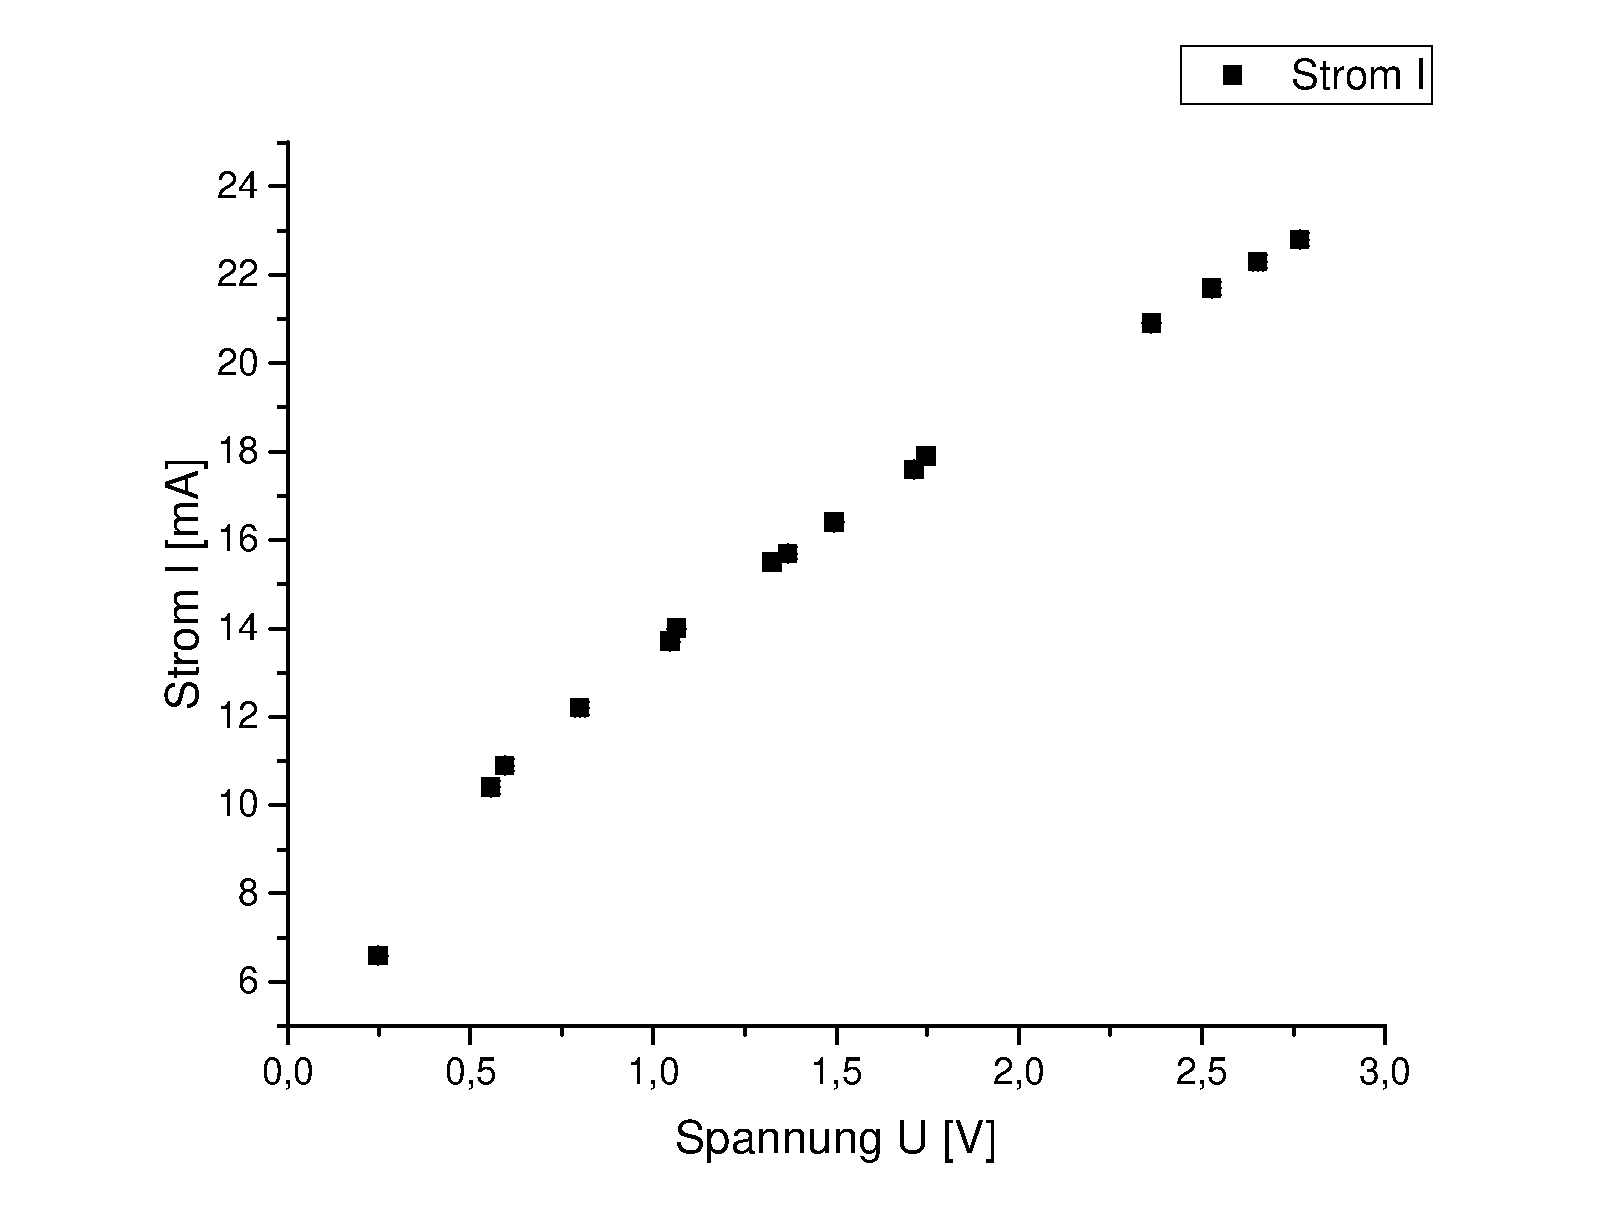
\includegraphics[width=0.7\textwidth]{Glueh_Kenn}
		\centering
		\caption{Hier ist die Stromstärke gegen die Spannung bei Betrieb einer Glühlampe aufgetragen. Die Unsicherheit ist kleiner als die Symbolgröße.}
		\label{Glueh_Kenn}
		\centering
	\end{figure}
	\begin{figure}[H]
		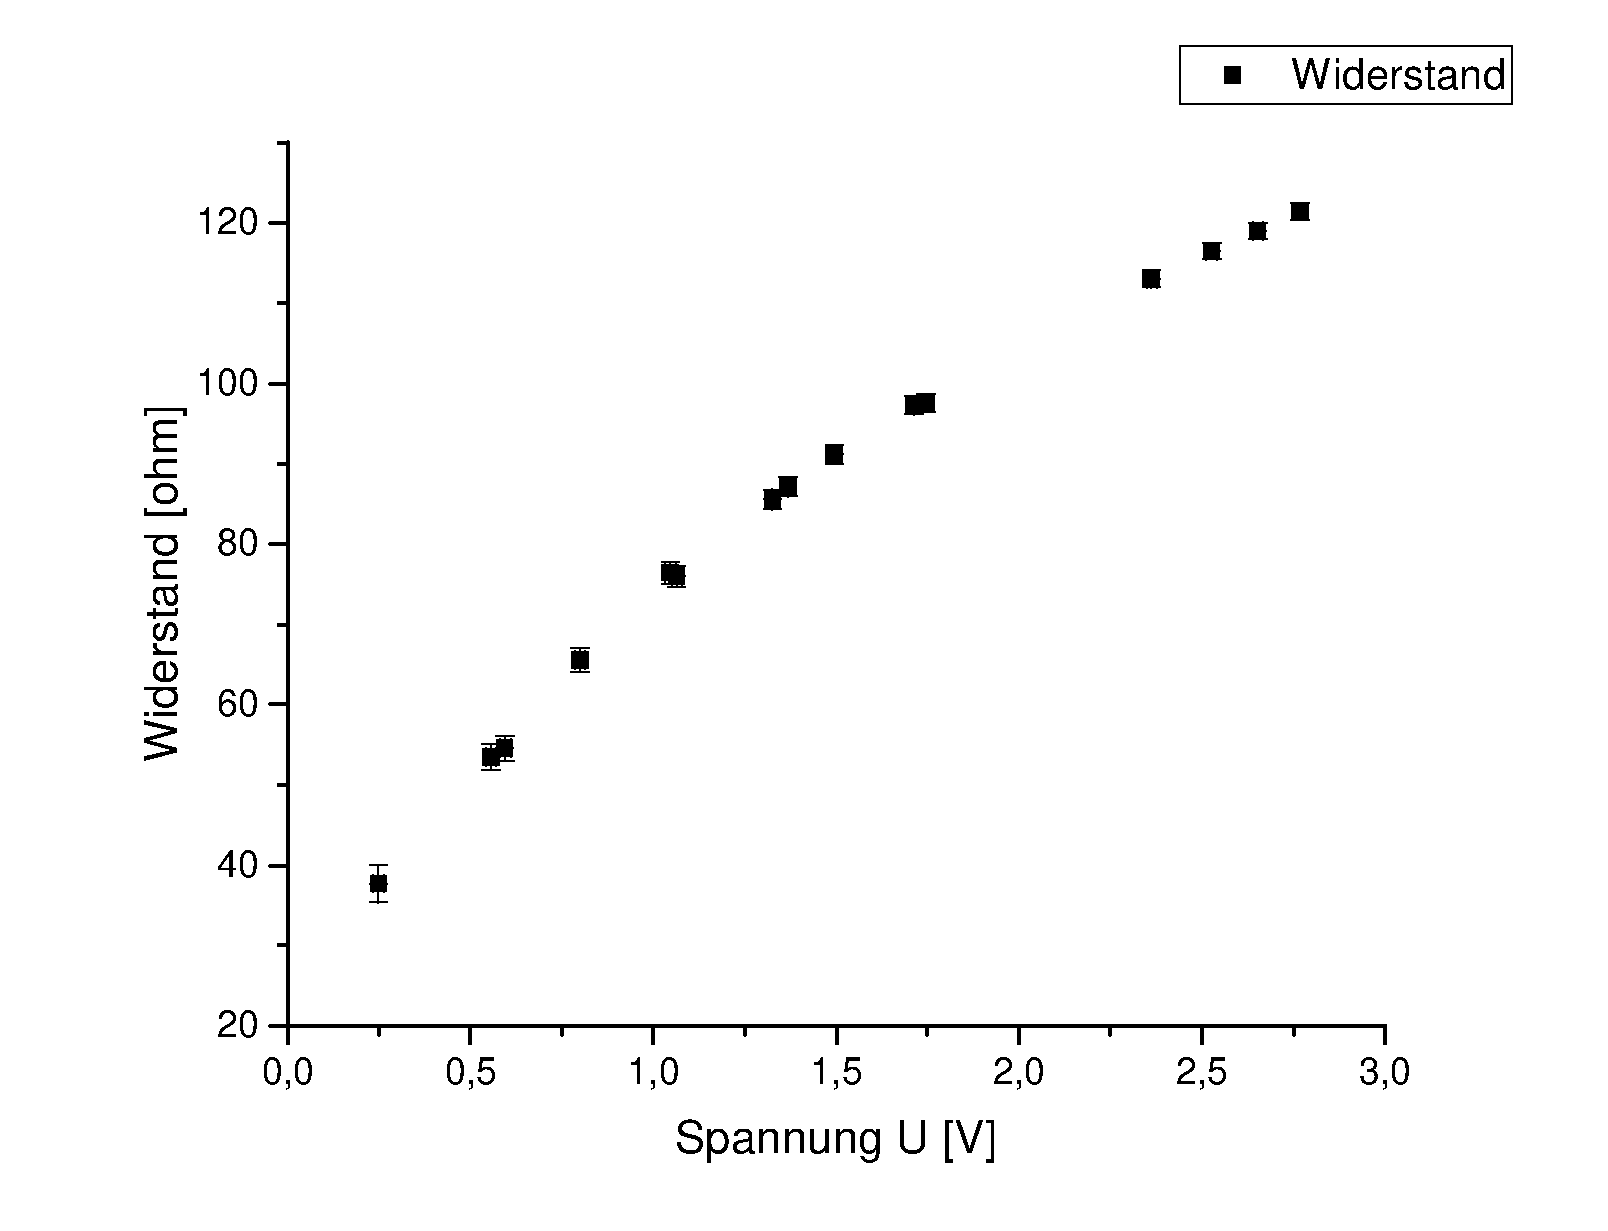
\includegraphics[width=0.7\textwidth]{Glueh_Wider}
		\centering
		\caption{Hier ist der Widerstand gegen die Spannung bei Betrieb einer Glühlampe aufgetragen. Die Unsicherheit ist kleiner als die Symbolgröße.}
		\label{Glueh_Wider}
		\centering
	\end{figure}
	Die aufgenommenen Kennlinie des NTC-Widerstands ist in \cref{ntc} dargestellt.
	\begin{figure}[H]
		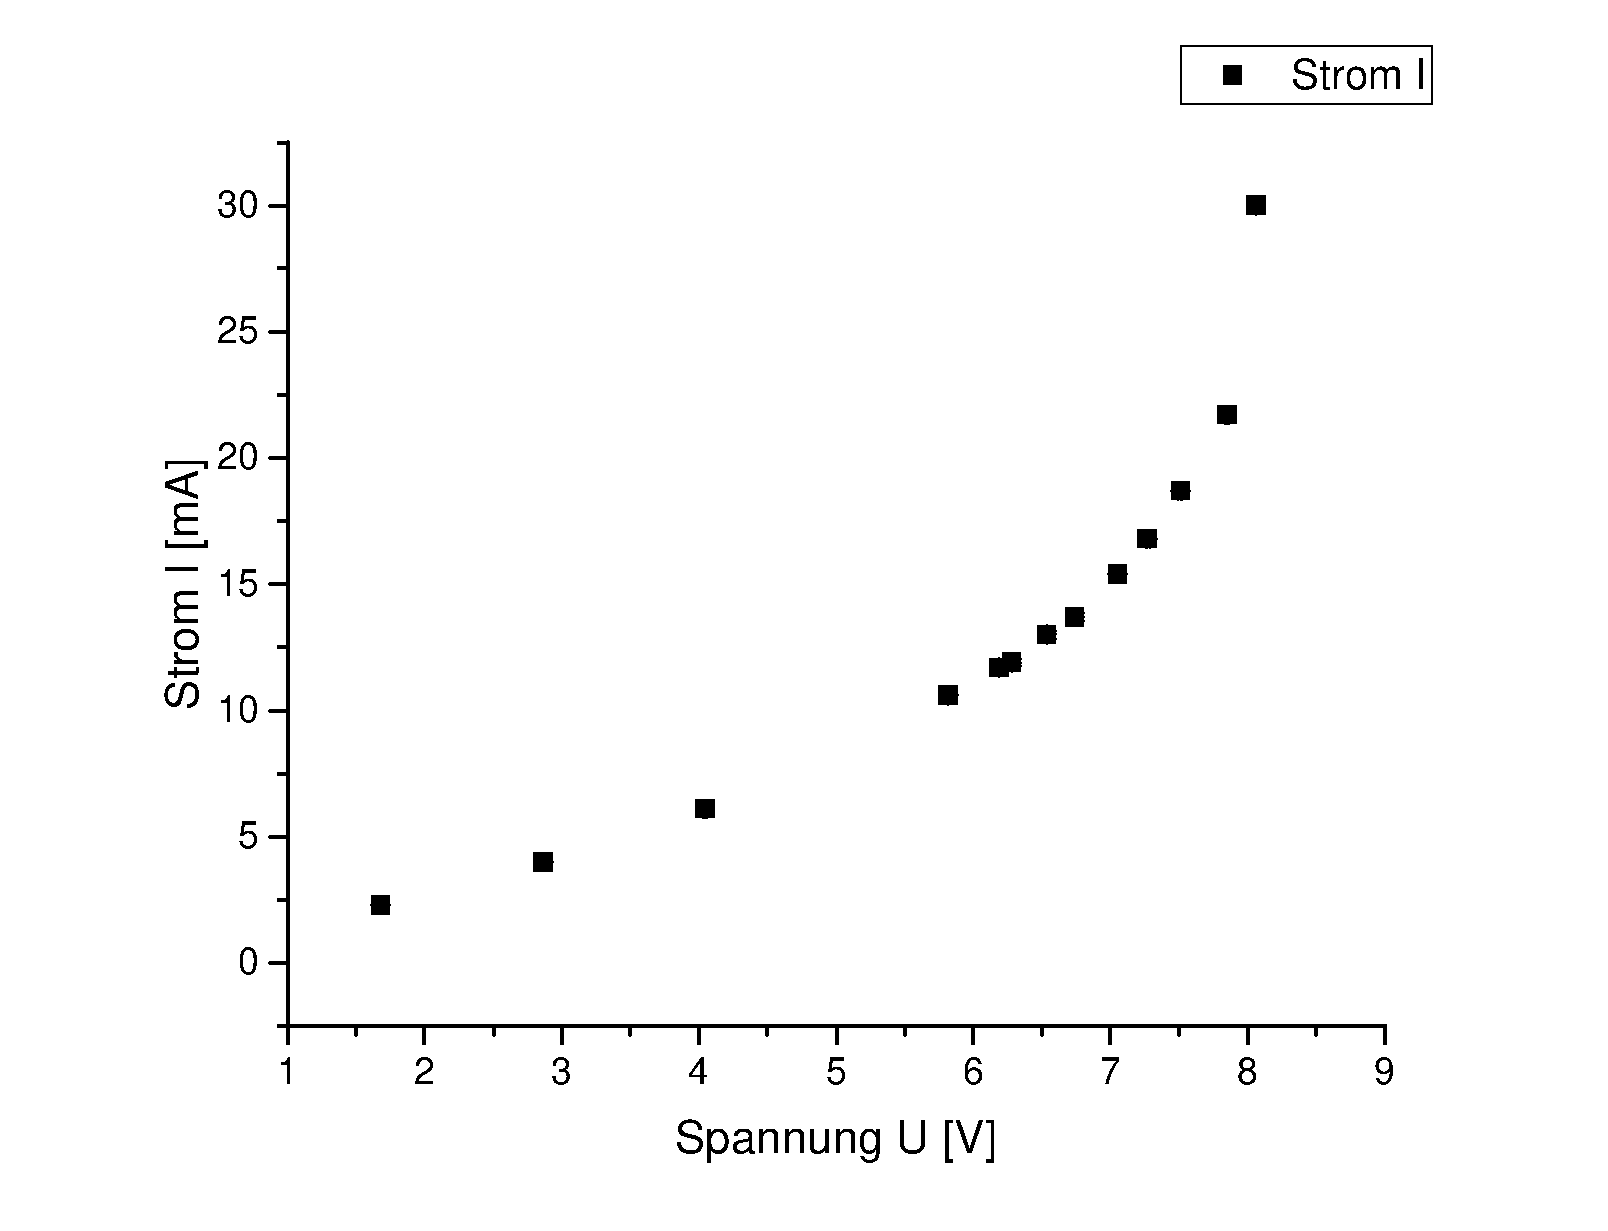
\includegraphics[width=0.7\textwidth]{ntc}
		\centering
		\caption{Hier ist der Widerstand gegen die Spannung bei Betrieb eines NTC-Widerstandes aufgetragen. Die Unsicherheit ist kleiner als die Symbolgröße.}
		\label{ntc}
		\centering
	\end{figure}
	Zuletzt soll die Glimmlampe betrachtet werden.
	Dazu wurde in \crefrange{glimm_steig}{glimm_fall} die Kennlinie für steigende bzw. fallende Spannungen dargestellt.
	Hieraus kann die Zünd- und Löschspannung der vorliegenden Glimmlampe bestimmt werden.
	Dazu wurde im Fall der Zündspannung der höchste Messwert gewählt, bei dem die Glimmlampe noch nicht zündete und das Messintervall als Fehler angenommen (mit rechteckiger WDF).
	Analog wurde die Löschspannung aus dem niedrigsten Messwert, bei dem die Glimmlampe noch leuchtete, bestimmt.
	Hier würde allerdings die Abtastrate gegen Unendlich gehen, da bei gleicher Spannung drei verschiedene Stromstärken gemessen wurden.
	Deshalb wurde für die Löschspannung stattdessen der Displayfehler gewählt, da die Messunsicherheit offensichtlich größer als die Abtastrate war.
	Dies ergibt eine Zündspannung von \SI{105\pm3,8}{V} und eine Löschspannung von \SI{84\pm 0,14}{V}.
	
	\begin{figure}[H]
		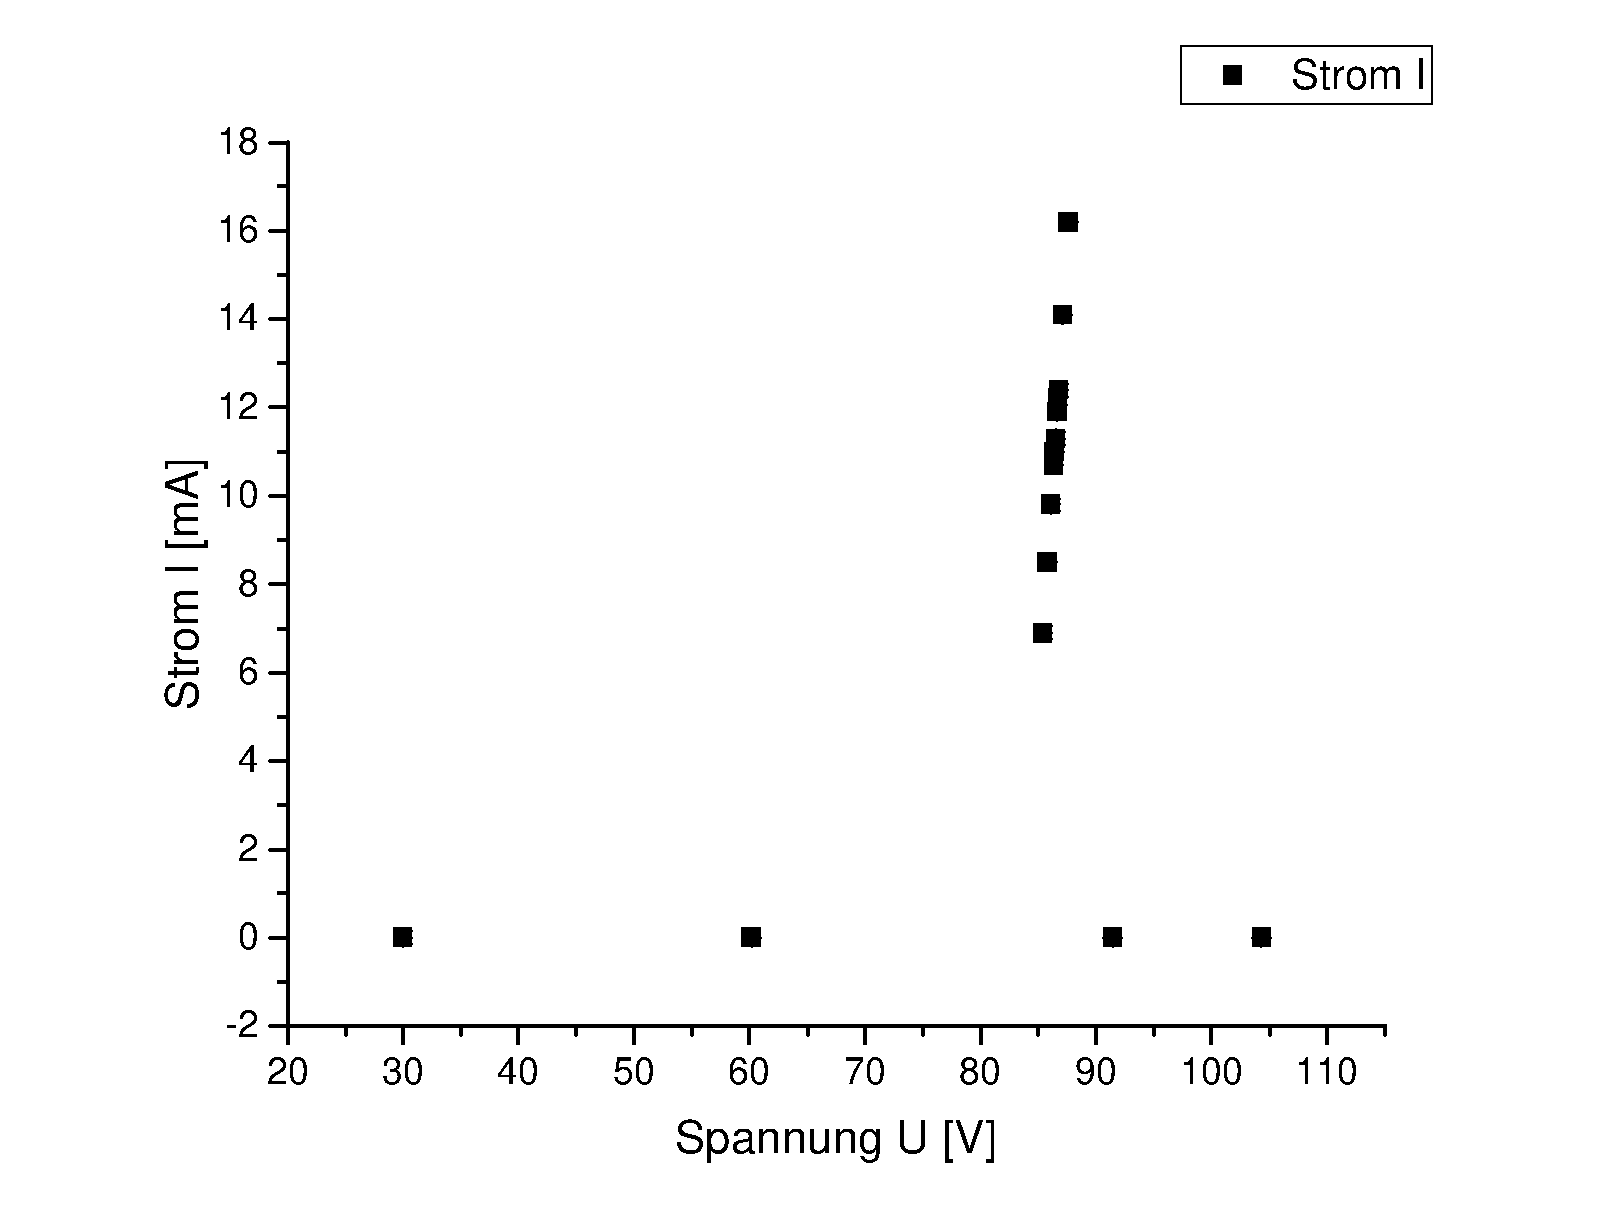
\includegraphics[width=0.7\textwidth]{glimm_steig}
		\centering
		\caption{Hier ist der Widerstand gegen die Spannung bei Betrieb einer Glimmlampe mit steigender Spannung aufgetragen. Die Unsicherheit ist kleiner als die Symbolgröße. Die Messwerte bei $I=0$ sind die Spannungen, bei denen die Glimmlampe noch nicht zündete, die also vor den Messwerten mit Stromstärken über null aufgezeichnet wurden.}
		\label{glimm_steig}
		\centering
	\end{figure}
	\begin{figure}[H]
		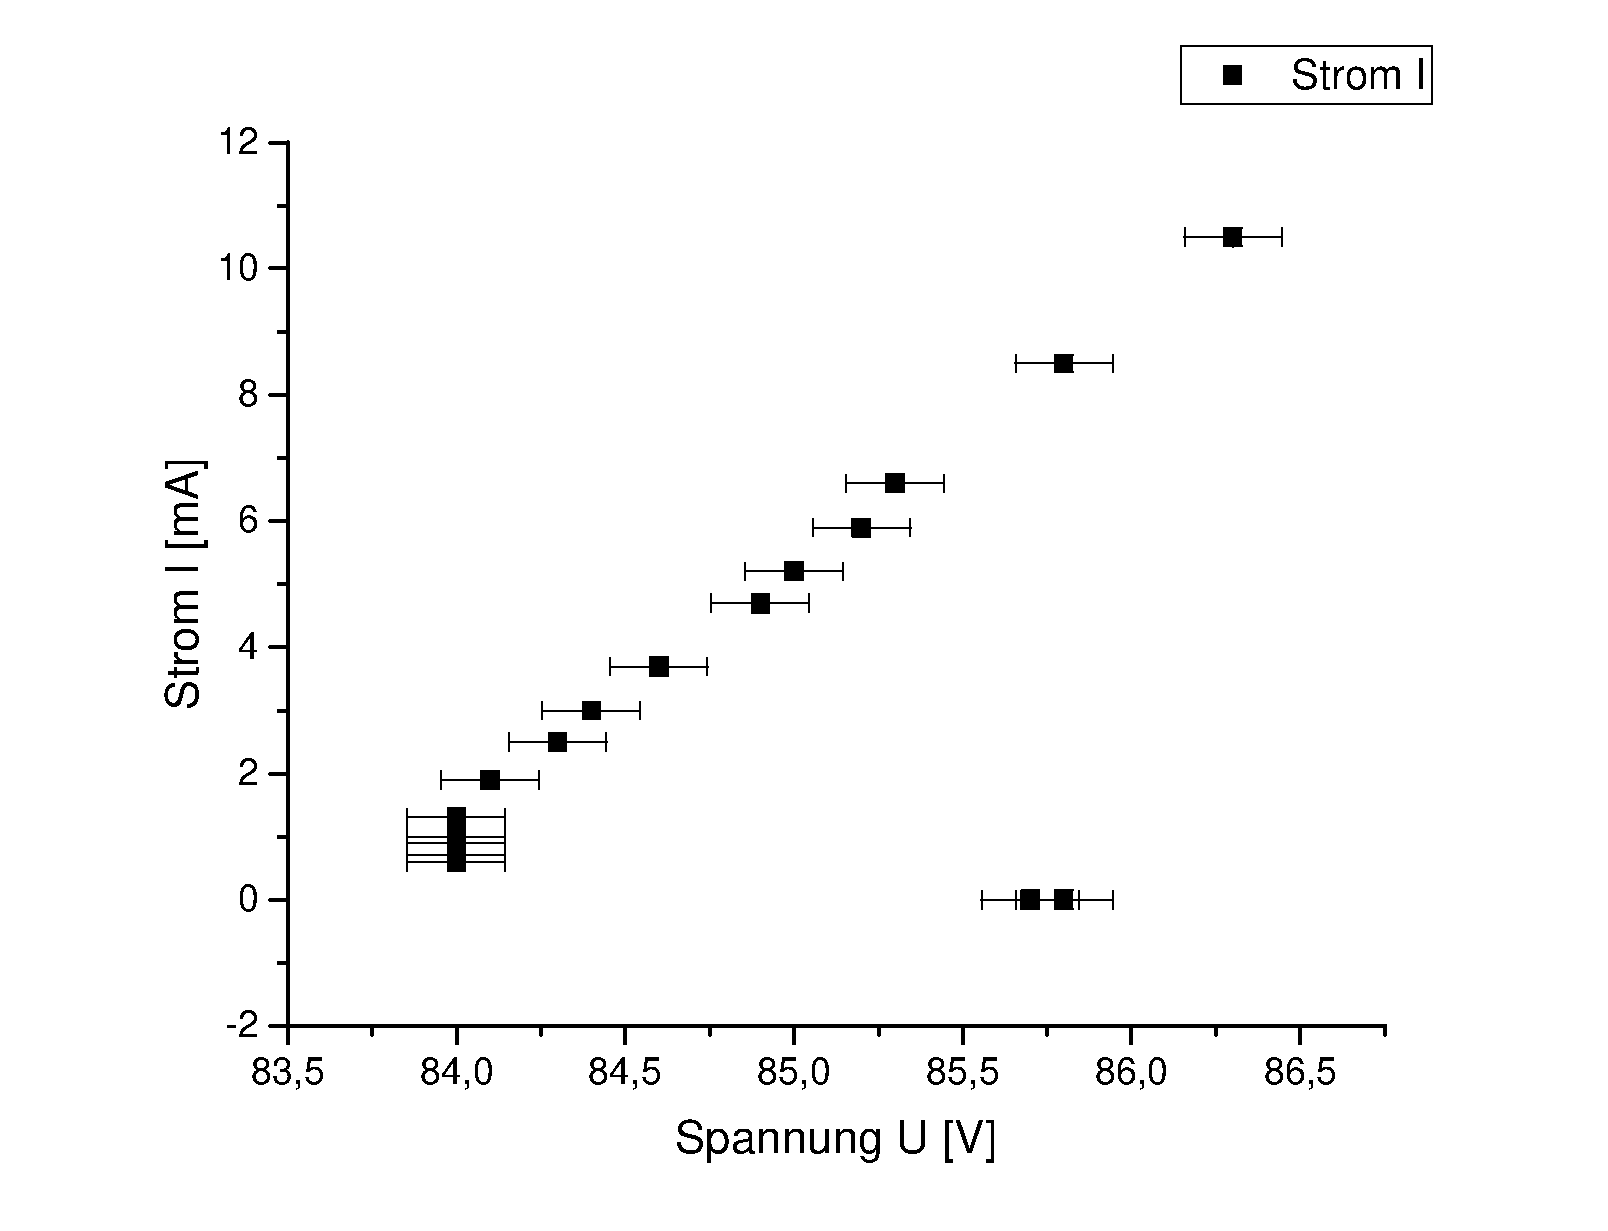
\includegraphics[width=0.7\textwidth]{glimm_fall}
		\centering
		\caption{Hier ist der Widerstand gegen die Spannung bei Betrieb einer Glimmlampe mit sinkender Spannung aufgetragen. Die Unsicherheit in y-Richtung ist kleiner als die Symbolgröße. Die Messwerte bei $I=0$ sind die Spannungen, bei denen die Glimmlampe erloschen war.}
		\label{glimm_fall}
		\centering
	\end{figure}
	\subsubsection{Temperatur-Widerstands-Charakteristik von Metalldraht}
	Aus der Wheatstoneschen Brückenschaltung (\cref{Wheatstone}) ergibt sich durch Anwendung der Kirchhoffschen Gesetze, wenn der verstellbare Widerstand so eingestellt ist, dass kein Strom fließt, der folgende Zusammenhang:
	\begin{equation}
		\frac{R_x(T)}{R_1}=\frac{R_\text{v}}{R_2}
	\end{equation}
	Dabei ist $R_1$ der zum positiven Pol der Stromquelle gewandte Teil des verstellbaren Widerstands und $R_2$ der zum negativen Pol gewandte.
	Angegeben waren die Größen $R_\text{ges}=R_2+R_1=\SI{11,3}{\ohm}$ und $R_\text{v}=\SI{5}{\ohm}$.
	Diese werden als exakt angenommen.
	Anhand der Skala des verstellbaren Widerstands wurde die Größe $a:=R_1/(R_2+R_1)$ gemessen.
	Hierfür wird eine Ableseunsicherheit von 0,0004 (Ableseintervall von 0,002 mit dreieckiger WDF) angenommen.
	Für den gesuchten Widerstand ergibt sich insgesamt:
	\begin{equation}
		R_x(T)=R_\text{v} \frac{R_1}{R_2}=R_\text{v} \frac{aR_\text{ges}}{R_\text{ges}(1-a)}=R_\text{v} \frac{a}{1-a}
	\end{equation}
	Die Unsicherheit von $R_x(T)$ ergibt sich gemäß \cref{Partielle_Unsicherheiten} aus der Unsicherheit von a:
	\begin{equation}
		u(R_x)= \frac{R_\text{v}}{(a-1)^2}
	\end{equation}
	Die Temperatur wurde mit einem Thermometer mit einer Digitalanzeige, die eine Nachkommastelle anzeigt, gemessen.
	Daraus folgt eine Unsicherheit von \SI{0,03}{\celsius}.
	In \crefrange{Temp_Steig}{Temp_Fall} ist der Widerstand $R_x$ des Kupferdrahtes gegen die Temperatur für steigende und fallende Temperaturen dargestellt.
	\par 
	Für den spezifischen Widerstand $\varrho $ gilt bei Temperaturen im Intervall von \SI{0}{\celsius} bis \SI{100}{\celsius}:
	\begin{equation}
		\varrho =\varrho_0 \left[ 1+\alpha (T-T_0) \right]
	\end{equation}
	Dies bedeutet, da $\varrho$ gemäß \cref{prop} proportional zu $R_x$ ist, dass die Steigung der Geraden im $R$-$T$-Diagramm dem Temperaturkoeffizienten $\alpha$ entspricht.
	Um den Temperaturkoeffizienten zu bestimmen, wurde ein linearer Fit mit dem Algorithmus von York durchgeführt.
	Die Ergebnisse aus diesem Fit sind in \cref{Koeff} dargestellt.
	%Da waren unterschiedliche Definitionen von alpha, die mMn nicht so ganz zusammenpassten von den Einheiten her und eig. ist das gelogen, aber Joey hat des auch so gemacht (nur in noch schlechter) Eigentlich wäre alpha mMn das da mal l/A, aber das kennt man ja beides net.
	\begin{equation}
	R_x =\varrho \frac{l}{A}
	\label{prop}
	\end{equation}
	\begin{figure}[H]
		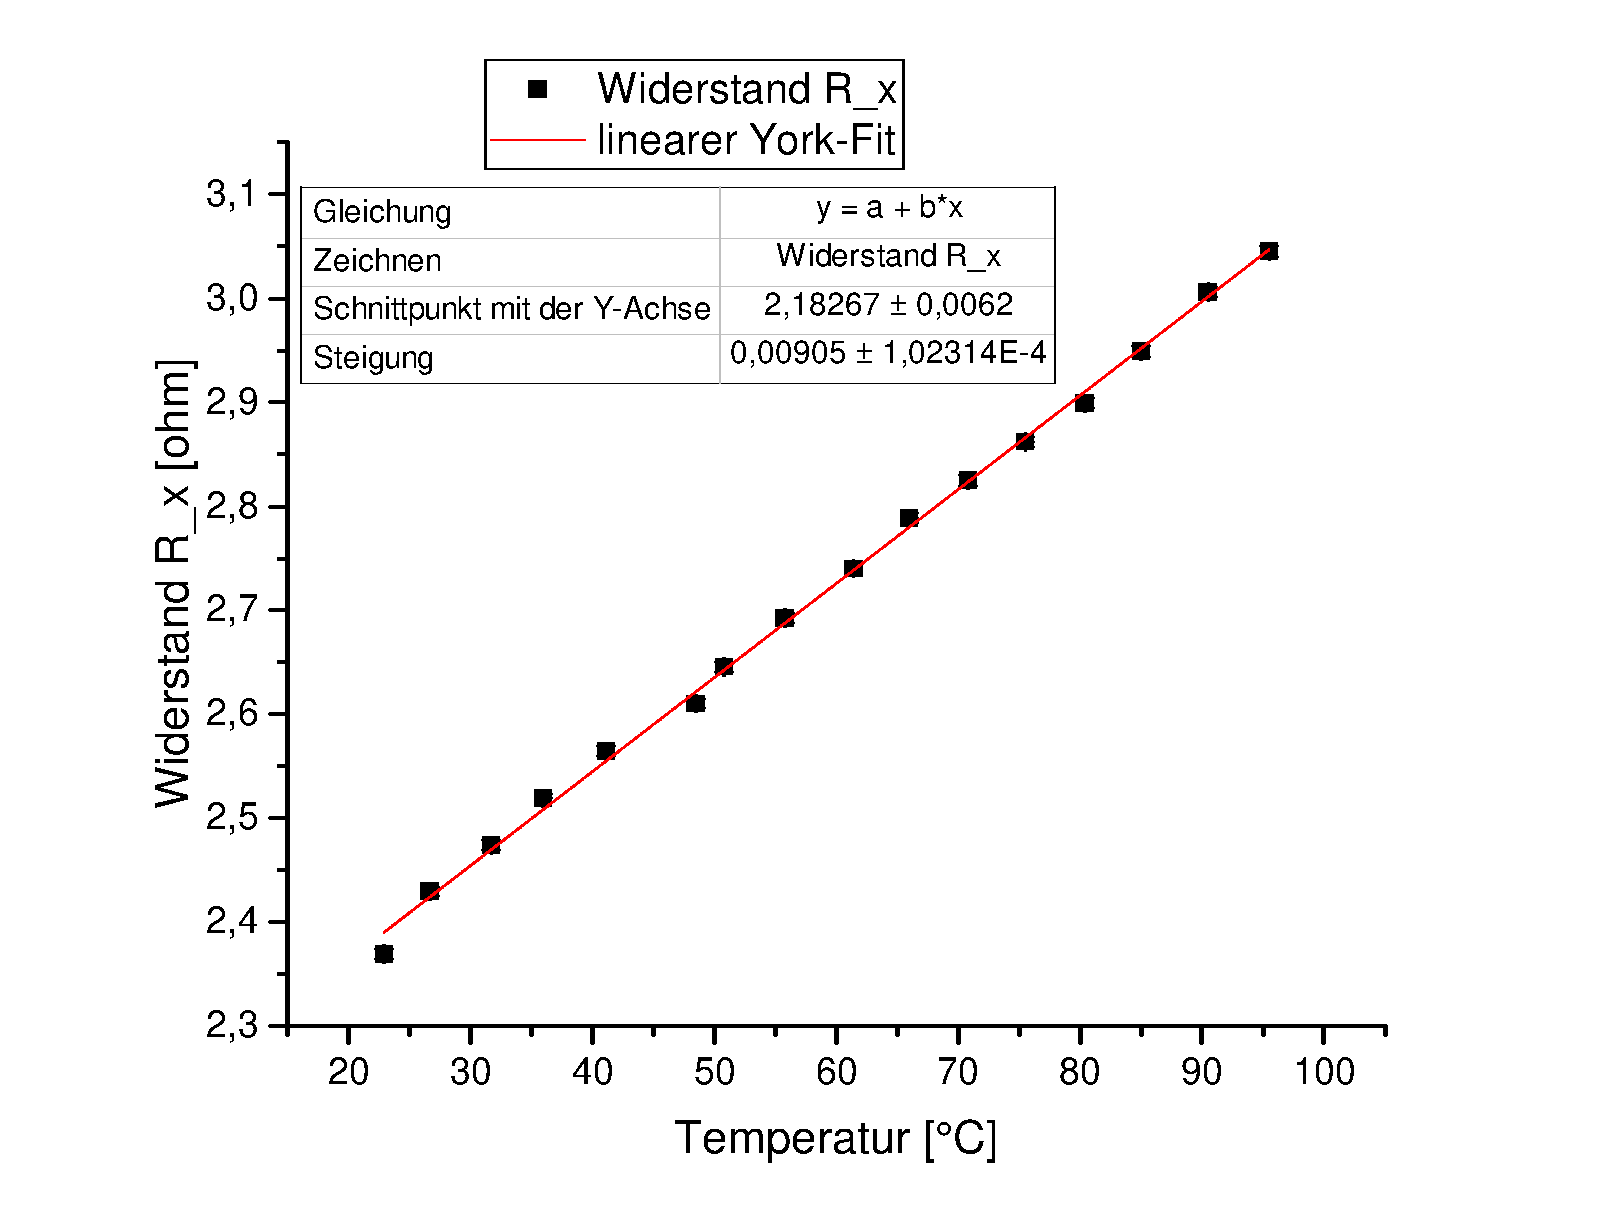
\includegraphics[width=0.7\textwidth]{Temp_Steig}
		\centering
		\caption{Der Widerstand des Kupferdrahtes aufgetragen gegen die Temperatur bei steigenden Temperaturen. Die Unsicherheit ist kleiner als die Symbolgröße.}
		\label{Temp_Steig}
		\centering
	\end{figure}
	\begin{figure}[H]
		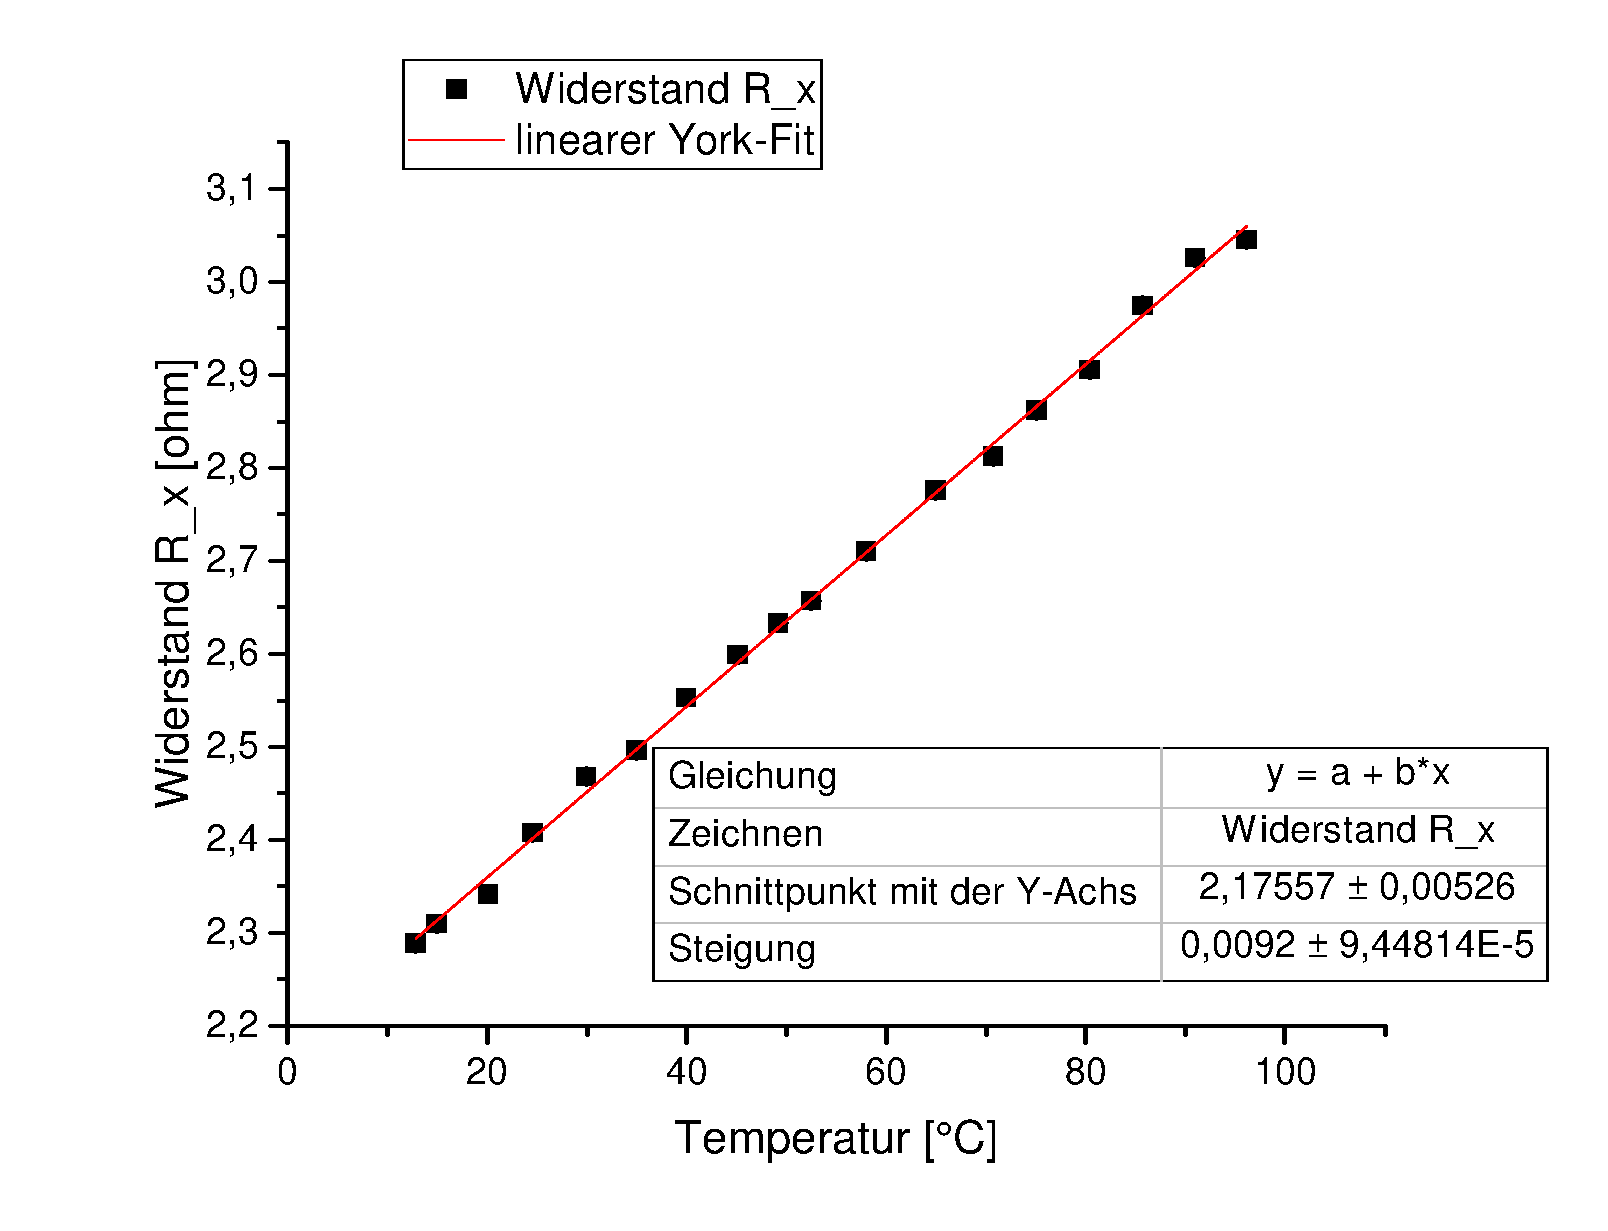
\includegraphics[width=0.7\textwidth]{Temp_Fall}
		\centering
		\caption{Der Widerstand des Kupferdrahtes aufgetragen gegen die Temperatur bei fallenden Temperaturen. Die Unsicherheit ist kleiner als die Symbolgröße.}
		\label{Temp_Fall}
		\centering
	\end{figure}
	\begin{table}[H]
		\centering
		\begin{tabular}{ r | c }
			&Temperaturkoeffizient \\ \hline
			Steigende Temperaturen& \SI{0,00905\pm 0,00011}{}\\
			Fallende Temperaturen & \SI{0,0092\pm 0,000095}{}\\
		\end{tabular}
		\caption{Die bei steigenden bzw. fallenden Temperaturen ermittelten Temperaturkoeffizienten.}
		\label{Koeff} 
	\end{table}
	\subsection{Diskussion}
	%TODO Bezug/Nutzten oder sonst was
	%TODO auch hier die Hypothese wiederholen
	Die Kennlinien der Dioden und der Glühlampe entsprechen den Erwartungen, bzw. der Hypothese, dass sie monoton ansteigen.
	Auch die Kennlinien des NTC-Widerstands deckt sich mit der Hypothese, dass der Widerstand mit der Temperatur abnimmt.
	Der Widerstand wird also durch den Stromfluss erhitzt und der Widerstand nimmt ab, wodurch sich der Stromfluss erhöht.
	In \cref{ntc} ergibt sich also eine exponentiell steigende Funktion.
	
	Die Lösch- und Zündspannungen der Glimmlampe entsprechen der Vermutung, dass die Löschspannung von \SI{84\pm 0,14}{V} kleiner als die Zündspannung von \SI{105\pm3,8}{V} ist.
	Zusätzlich lässt sich die Hypothese der direkten Temperaturabhängigkeit des Metalldrahts bestätigen, da sich bei steigender und fallender Temperatur überschneidende Unsicherheitsintervalle für den Temperaturkoeffizienten $\alpha$ ergaben.
	Für steigende Temperaturen haben wir ein $\alpha$ von \SI{0,00905\pm 0,00011}{} und für fallende von \SI{0,0092\pm 0,000095}{} gemessen.
	
	\section{Schlussfolgerung}
	Alle aufgeführten Hypothesen konnten bestätigt werden.
	Die Stromstärke stieg bei allen Bauteilen monoton mit der Spannung an.
	Der NTC-Widerstand nahm mit der Temperatur (durch selbstständiges Erhitzten bei Stromfluss) ab.
	Die Löschspannung der Glimmlampe ist kleiner als ihre Zündspannung.
	Der ermittelte Temperaturkoeffizient des Metalldrahts ist unabhängig davon, ob man im Vorgang des Erhitzens oder des Abkühlens misst.
	Um die Zünd- und Löschspannung genauer bestimmen zu können, müssten mehrere Messungen durchgeführt werden und die Messpunkte weit entfernt von den unstetigen Sprüngen der Stromstärken wären nicht weiter relevant.
	%TODO Rückgriff auf Hypothese und drittes Nennen dieser
	
	%TODO Quellen zitieren, Websiten mit Zugriffsdatum
	%TODO Verweise auf das Laborbuch (sind erlaubt)
	%TODO Tabelle + Bilder mit Beschriftung
	\printbibliography
\end{document}
